\chapter{Cryptography in Telecoms: GSM, LTE, and 5G}

Every other chapter in this book has assumed a comfortable setting: two computers with spare cycles, a fresh connection, the freedom to run a Diffie-Hellman exchange or verify a certificate chain before sending a single byte of data. Cellular telephony grew up in a harsher world. The first digital mobile standard, GSM, was designed in the late 1980s for handsets with the compute budget of a pocket calculator, a radio link that drops packets for fun, and a regulatory environment where strong cryptography was treated as a munition. The cryptographers who built it were not fools. They were boxed in, and you can read every constraint of the time directly off the cipher they shipped.

This chapter follows mobile security across three generations. We start with GSM (2G): how a SIM card proves who you are, how the A5 family of stream ciphers scrambles the air interface, and why both were broken so thoroughly that you can decrypt a GSM call today with a laptop and a rainbow table. Then we meet the Authentication and Key Agreement protocol -- AKA -- introduced in 3G and carried forward, with steady repairs, into LTE (4G) and 5G. The throughline is a single recurring villain: the \emph{IMSI catcher}, a fake base station that lifts your identity out of the air and, in the GSM era, your conversation too. Each generation closes one more door on that attacker. 5G finally shuts the last obvious one by encrypting your permanent identity before it ever leaves the phone.

The reason telecom crypto deserves its own chapter is that it is the largest deployed cryptosystem on Earth -- billions of SIM cards, every one a tamper-resistant token holding a symmetric key -- and because its history is the cleanest available case study in how real-world constraints, export law, and backward compatibility shape a design, sometimes fatally.

\section{The setting: who is who, and what they trust}
\label{ch29:setting}

Before any cipher, fix the cast. A mobile network has more named parties than our usual Alice and Bob, and the trust relationships are the whole story.

\begin{itemize}
  \item The \textbf{subscriber}, carrying a \textbf{handset} (the phone, called \emph{Mobile Equipment} or ME in the specs) into which a \textbf{SIM} card is inserted. The SIM is a small tamper-resistant smartcard. It is the cryptographic root of the subscriber's identity.
  \item The \textbf{home network} -- the operator you pay. Deep inside it sits a database, historically the \emph{Authentication Centre} (AuC), that holds the master secret key for every SIM it ever issued.
  \item The \textbf{visited network} -- the operator whose tower you are actually camped on right now, which may not be your home network (this is roaming). The tower itself is the \emph{base station} (BTS in GSM, eNodeB in LTE, gNodeB in 5G).
  \item \textbf{Eve}, who owns a radio. In the cellular threat model Eve is unusually powerful, because she can do more than listen. She can transmit. A radio that transmits the right beacons can impersonate a base station, and a phone has historically had no way to tell a real tower from a fake one.
\end{itemize}

\begin{intuitionbox}
The single fact that organizes all of telecom security is this: \textbf{the SIM and the home network share a secret symmetric key $K_i$, and nobody else ever learns it -- not even the visited network you are roaming on.} The SIM is manufactured with $K_i$ burned in; the same $K_i$ is recorded in the operator's AuC. From the day the card is printed, those two endpoints share a 128-bit secret that never travels over any wire or any radio. Everything else -- authentication, the per-call encryption key, identity protection -- is bootstrapped from that one pre-shared symmetric key.

This is a very different starting point from TLS. TLS strangers establish a key from nothing using public-key cryptography. Cellular subscribers are not strangers to their operator; they were provisioned. So telecom can lean on cheap, fast symmetric primitives -- no modular exponentiation on a 1990 SIM -- at the cost of a logistics problem (printing and protecting billions of keys) that TLS does not have.
\end{intuitionbox}

\begin{figure}[H]
\centering
\begin{tikzpicture}[font=\small,node distance=8mm]
  \node[draw,rounded corners,fill=aliceblue!12,minimum width=22mm,minimum height=10mm] (sim) {SIM};
  \node[draw,rounded corners,right=22mm of sim,minimum width=22mm,minimum height=10mm] (me) {Handset};
  \node[draw,rounded corners,right=34mm of me,fill=evered!12,minimum width=22mm,minimum height=10mm] (bts) {Base station};
  \node[draw,rounded corners,right=22mm of bts,fill=bobgreen!12,minimum width=26mm,minimum height=10mm] (home) {Home / AuC};
  \node[draw,dashed,fit=(sim)(me),inner sep=4mm,label=below:{the phone you hold}] {};
  \draw[<->,thick] (me) -- (bts) node[midway,above]{radio (Eve listens here)};
  \draw[<->,thick] (bts) -- (home) node[midway,above]{operator backbone};
  \draw[<->,dashed,structurepurple,thick] (sim.north) to[bend left=32] node[midway,above,structurepurple]{shared $K_i$ (never transmitted)} (home.north);
\end{tikzpicture}
\caption{The trust map. The secret $K_i$ lives only on the SIM and in the home network's AuC. The vulnerable link is the radio between handset and base station.}
\label{ch29:fig-trustmap}
\end{figure}

\section{GSM authentication: a challenge and a response}
\label{ch29:gsm-auth}

When your GSM phone first contacts a tower, two things must happen before you can place a call. The network must be convinced the SIM is genuine (authentication), and both sides must derive a session key to encrypt the radio link (key agreement). GSM does both with a single challenge--response built on the shared $K_i$.

Here is the dance, with the concrete names from the standard.

\begin{enumerate}
  \item The phone announces an identity to the tower. Ideally a temporary one (the TMSI, discussed below), but on a first contact, or when the network asks, it sends its permanent identity, the \textbf{IMSI} (International Mobile Subscriber Identity -- the number that uniquely names your SIM).
  \item The visited network forwards the IMSI to the home network and asks for an \emph{authentication triplet}. The home AuC looks up $K_i$, generates a fresh random 128-bit challenge \textbf{RAND}, and computes two values with secret algorithms that take $(K_i, \text{RAND})$ as input:
  \[
    \text{SRES} = A3(K_i, \text{RAND}) \in \set{0,1}^{32},
    \qquad
    K_c = A8(K_i, \text{RAND}) \in \set{0,1}^{64}.
  \]
  SRES is a 32-bit \emph{signed response}; $K_c$ is the 64-bit session key for encryption. The home network ships the triplet $(\text{RAND}, \text{SRES}, K_c)$ to the visited network and keeps $K_i$ to itself.
  \item The visited network sends RAND over the air to the phone. The SIM, which also holds $K_i$, computes its own $A3(K_i,\text{RAND})$ and $A8(K_i,\text{RAND})$, getting SRES$'$ and $K_c$.
  \item The phone returns SRES$'$. The network checks SRES$' \stackrel{?}{=}$ SRES. If they match, the SIM has proven it knows $K_i$ without ever revealing it, and both sides now hold the same $K_c$ to encrypt the call with the A5 cipher.
\end{enumerate}

\begin{whybox}
Why is this an authentication? RAND is fresh and unpredictable, so a recorded old (RAND, SRES) pair is useless against a new challenge -- this defeats replay. Producing the correct SRES requires $K_i$; an attacker who does not know $K_i$ can do no better than guess a 32-bit value, succeeding with probability $2^{-32}$. And $K_i$ never crosses the radio, so passive eavesdropping on the exchange does not leak it (assuming $A3$ does not).

Why is the key agreement ``free''? $K_c = A8(K_i,\text{RAND})$ is a deterministic function of the shared secret and the public nonce, so both endpoints compute the identical $K_c$ without transmitting it. RAND is public; $K_i$ is shared; therefore $K_c$ is shared. The eavesdropper sees RAND but, lacking $K_i$, cannot compute $K_c$. This is the symmetric-key analogue of a key exchange: not Diffie-Hellman, just ``run a PRF on a common secret and a common nonce.''
\end{whybox}

In practice operators implement $A3$ and $A8$ together as a single algorithm called \textbf{COMP128}, which takes $(K_i, \text{RAND})$ and emits 128 bits: the first 32 are SRES, and 64 of the rest become $K_c$ (with, as we will see, a fatal twist).

\begin{figure}[H]
\centering
\begin{tikzpicture}[font=\small]
  \node (sim) at (0,0) {\textbf{SIM} (has $K_i$)};
  \node (net) at (8.5,0) {\textbf{Network} (has triplet)};
  \draw[thick] (sim) -- (0,-4.6);
  \draw[thick] (net) -- (8.5,-4.6);
  \draw[->,thick] (0,-0.7) -- node[above,sloped]{IMSI / TMSI} (8.5,-0.95);
  \draw[->,thick] (8.5,-1.6) -- node[above,sloped]{RAND (128-bit nonce)} (0,-1.85);
  \node[align=center,structurepurple] at (4.25,-2.55) {SIM computes SRES$'=A3(K_i,\text{RAND})$,\ $K_c=A8(K_i,\text{RAND})$};
  \draw[->,thick] (0,-3.1) -- node[above,sloped]{SRES$'$ (32 bits)} (8.5,-3.35);
  \node[align=center] at (4.25,-3.95) {network checks SRES$'\stackrel{?}{=}$SRES; if ok, encrypt with $K_c$};
\end{tikzpicture}
\caption{GSM challenge--response. Only RAND and the 32-bit SRES cross the air. Note the asymmetry: the phone never checks the network.}
\label{ch29:fig-gsm-auth}
\end{figure}

\begin{trapbox}
Read figure~\ref{ch29:fig-gsm-auth} again and find the missing arrow. The network challenges the phone, but \emph{the phone never challenges the network}. GSM authentication is \textbf{one-way}: the SIM proves itself to the tower, the tower proves nothing to the SIM. A phone will obediently camp on, authenticate to, and encrypt toward any device that speaks the protocol and tells it to. This single asymmetry is the root of the IMSI-catcher problem, and fixing it is the main job of 3G/4G/5G AKA. Hold that thought.
\end{trapbox}

\subsection{A worked triplet with tiny numbers}
\label{ch29:gsm-toy}

COMP128 is too large to trace by hand, but the \emph{structure} of challenge--response is just a keyed function evaluated on a nonce, and we can build a toy that behaves the same way. Let our toy keyed function be
\[
  F(K,x) = (3\,K + 7\,x + 11) \bmod 256,
\]
a deliberately weak stand-in for $A3/A8$ over the ring $\Zn{256}$. Suppose the SIM and AuC share $K_i = 100$.

The AuC picks a random challenge, say $\text{RAND} = 42$. It computes a ``response'' and ``key'' from two slices; to keep it tiny we will say
\[
  \text{SRES} = F(100, 42) = (300 + 294 + 11)\bmod 256 = 605 \bmod 256 = 93,
\]
\[
  K_c = F(100, 43) = (300 + 301 + 11)\bmod 256 = 612 \bmod 256 = 100 .
\]
The AuC ships the triplet $(\text{RAND}, \text{SRES}, K_c) = (42, 93, 100)$ to the visited network and keeps $K_i=100$. The tower forwards $\text{RAND}=42$ to the phone. The SIM, holding $K_i=100$, recomputes $F(100,42)=93$ and returns SRES$'=93$. The tower checks $93 = 93$: pass. Both sides now share $K_c = 100$ as the session key, having transmitted only the public nonce $42$ and the response $93$. An eavesdropper who saw $(42, 93)$ but does not know $K_i$ cannot recover $K_c = 100$.

\begin{trapbox}
Our toy $F$ is linear, so an attacker who captures one pair $(\text{RAND},\text{SRES})$ can solve for $K$ immediately. From $\text{SRES} \equiv 3K + 7\,\text{RAND} + 11 \pmod{256}$ we get $3K \equiv \text{SRES} - 7\,\text{RAND} - 11 \pmod{256}$. Since $\gcd(3,256)=1$, multiply by $3^{-1}\equiv 171 \pmod{256}$ and recover $K$ from a \emph{single} captured challenge--response. Real $A3/A8$ must be a one-way, nonlinear function precisely so that this cannot happen. COMP128's first version failed at exactly this kind of structural weakness -- the next section shows how.
\end{trapbox}

\section{Where GSM broke: COMP128, A5/1, and A5/2}
\label{ch29:gsm-breaks}

GSM's cryptography is a museum of how not to do it, and the exhibits are worth studying because each failure has a clean cause.

\subsection{COMP128-1: cloning the SIM}
\label{ch29:comp128}

The original $A3/A8$ algorithm, COMP128-1, was secret -- ``security through obscurity'' -- but leaked and was reverse-engineered in 1998 by Briceno, Goldberg, and Wagner. Its compression function had a collision weakness: certain pairs of RAND inputs that differed only in a few bytes produced internal collisions that the attacker could detect from the outputs. By choosing on the order of $2^{17}$ to $2^{19}$ carefully crafted RAND challenges and feeding them to a SIM (you need physical access, or a fake base station that keeps issuing challenges), an attacker could solve for $K_i$ a few bits at a time.

\begin{attackbox}
\textbf{SIM cloning via the COMP128-1 chosen-challenge attack.} The 128-bit $K_i$ is recovered in small groups. The attacker queries the SIM with chosen RANDs designed to collide in the second round of COMP128's butterfly structure; a collision in the output narrows two key bytes at a time. Roughly $2^{18}$ queries -- a few hours over the SIM's slow smartcard interface -- and $K_i$ falls. With $K_i$ in hand the attacker writes it to a blank programmable SIM and now owns a perfect clone: it authenticates as you, places calls billed to you, and can decrypt your traffic. The fix was COMP128-2 and -3 (collision-resistant, still secret) and, properly, operator-specific algorithms built on a public, vetted primitive (the MILENAGE construction over AES, used in 3G+). The lesson is the oldest one in the book: do not roll a secret cipher and hope nobody looks.
\end{attackbox}

\subsection{The A5 family: the cipher on the air}
\label{ch29:a5}

Once $K_c$ is agreed, the call's voice frames are encrypted with a stream cipher from the A5 family. There were three relevant variants:

\begin{itemize}
  \item \textbf{A5/1} -- the ``strong'' version, for Western Europe and North America. A hardware-efficient stream cipher built from three linear-feedback shift registers (LFSRs).
  \item \textbf{A5/2} -- a deliberately weakened version for export to markets where regulators forbade strong crypto. It was designed to be breakable.
  \item \textbf{A5/0} -- no encryption at all. Plaintext over the air. Selectable by the network.
\end{itemize}

A5/1 takes the 64-bit $K_c$ and a 22-bit publicly-known frame number (the count of which 114-bit GSM burst you are on) and produces a keystream that is xored into the voice frame, exactly the stream-cipher construction of the stream-cipher chapter: $c = m \xor \text{keystream}(K_c, \text{frame})$. The frame number is the nonce that keeps each burst's keystream distinct so you do not get the two-time-pad disaster.

\begin{figure}[H]
\centering
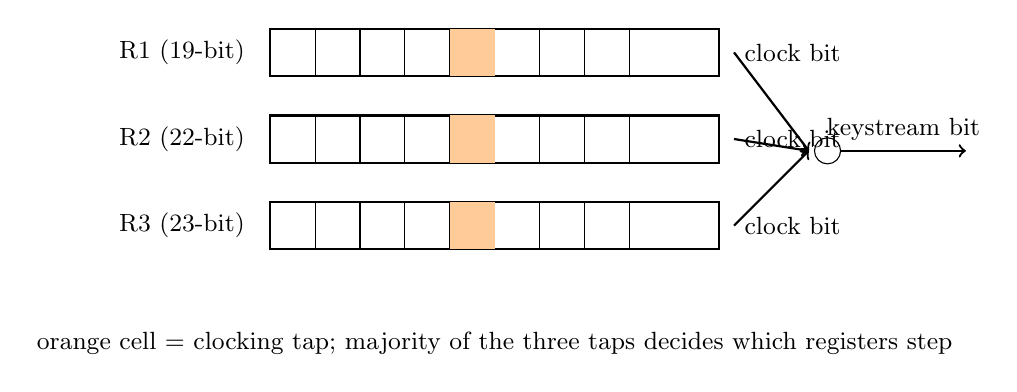
\begin{tikzpicture}[font=\small,xscale=0.95]
  \foreach \y/\n/\len in {0/R1/19, -1.1/R2/22, -2.2/R3/23}{
    \draw[thick] (0,\y) rectangle (6,\y+0.6);
    \foreach \x in {1,...,8}{\draw (0.6*\x,\y) -- (0.6*\x,\y+0.6);}
    \node[left=2mm] at (0,\y+0.3) {\n\ (\len-bit)};
    \node[right=2mm] at (6,\y+0.3) {\small clock bit};
    \fill[orange!40] (2.4,\y) rectangle (3.0,\y+0.6);
  }
  \node[align=left] at (3,-3.4) {orange cell = clocking tap; majority of the three taps decides which registers step};
  \draw[->,thick] (6.2,0.3) -- (7.2,-0.95);
  \draw[->,thick] (6.2,-0.8) -- (7.2,-0.95);
  \draw[->,thick] (6.2,-1.9) -- (7.2,-0.95);
  \node[draw,circle] (xor) at (7.45,-0.95) {$\xor$};
  \draw[->,thick] (xor) -- node[above]{keystream bit} (9.3,-0.95);
\end{tikzpicture}
\caption{A5/1: three LFSRs of lengths 19, 22, 23 (total 64 bits = $K_c$). The output bit is the xor of the three top bits; majority-rule clocking decides which registers advance each step.}
\label{ch29:fig-a51}
\end{figure}

The clever bit in A5/1 is the irregular, majority-rule clocking: each register has a designated clocking tap, the majority value among the three taps is computed, and only registers whose clocking tap agrees with the majority step forward. This nonlinear clock control is what stops the cipher from being a trivial linear system. It is not enough.

\begin{attackbox}
\textbf{Breaking A5/1.} A5/1 has been broken many times over, each break cheaper than the last.
\begin{itemize}
  \item \emph{Time--memory tradeoff (Biryukov--Shamir--Wagner, 2000; Barkan--Biham--Keller).} The 64-bit internal state is small enough to attack with precomputation. The keystream for parts of a call is partly predictable (frames carry known structure), giving known keystream. With a few seconds of known keystream you look up the state in a precomputed table.
  \item \emph{The A5/1 Cracking Project (Nohl et al., 2009).} Karsten Nohl's team publicly computed about 2 TB of rainbow tables for A5/1. With those tables and a cheap software radio capturing a call, $K_c$ is recovered in seconds to minutes on a PC. The point was political: to prove the cipher was dead and shame operators into upgrading.
  \item \emph{Key length.} Even ignoring structural flaws, $K_c$ is 64 bits -- and in many deployments the 10 least-significant bits were forced to zero, leaving 54 bits of effective key. A brute force over $2^{54}$ is within reach of a modest GPU farm.
\end{itemize}
\end{attackbox}

\begin{attackbox}
\textbf{A5/2 is broken in real time -- and it poisons A5/1.} A5/2 was built to be weak, and Barkan, Biham, and Keller (2003) showed it falls to a ciphertext-only attack in well under a second: the cipher is so linear that a handful of frames let you solve for the state by linear algebra. The deeper sting is the \emph{cross-protocol attack}. Recall $K_c$ is derived from $(K_i,\text{RAND})$ \emph{independent of which A5 variant will use it}. So an active attacker (an IMSI catcher) replays a captured RAND to the victim, but forces the phone to use A5/2, instantly recovers $K_c$ from the A5/2 traffic, and now holds the very same $K_c$ that the victim used for a real A5/1 call with the legitimate network. The weak cipher's key \emph{is} the strong cipher's key. One rotten variant compromises the whole suite. The repair: A5/2 was prohibited in handsets from 2006 onward, and modern phones refuse it.
\end{attackbox}

\begin{historybox}
Why ship a cipher you know is weak? Cold-war and 1990s export controls. Cryptography was regulated as a munition under regimes like COCOM and the US ITAR; ``strong'' crypto could not be exported to many countries. A5/1 was the NATO-region cipher; A5/2 was the deliberately enfeebled export cipher so that GSM phones could be sold worldwide while keeping intercept capability for the exporting states. The same political pressure explains the truncated effective key length. The technology outlived the politics, and the weakness outlived its purpose -- which is the recurring tragedy of mandated weakness: the back door does not know who is walking through it.
\end{historybox}

\subsection{The arithmetic of a 54-bit key}
\label{ch29:a5-numbers}

Put numbers on why $K_c$'s key length matters, because the gap between 64 and 54 bits is not a rounding error -- it is the difference between ``barely standing'' and ``already fallen.'' Take the deployments that forced the low 10 bits of $K_c$ to zero, leaving $2^{54}$ effective keys. Suppose a brute-force rig tries $2^{30}$ candidate A5/1 states per second (a billion per second, a plausible figure for a small GPU cluster checking each state against a few frames of known keystream). Then

\[
  \frac{2^{54}}{2^{30}} = 2^{24} \text{ seconds} \approx 1.68\times 10^{7}\ \text{s} \approx 194\ \text{days}.
\]

That is a single rig, brute over the whole reduced space, in well under a year -- and the expected time to a hit is half that, about 97 days. Now compare the full 64-bit key:

\[
  \frac{2^{64}}{2^{30}} = 2^{34} \text{ seconds} \approx 1.72\times 10^{10}\ \text{s} \approx 545\ \text{years}.
\]

The 10 forced bits bought the attacker a factor of $2^{10} = 1024$, collapsing five centuries into a few months. And this is the \emph{naive} attack. The time--memory tradeoff changes the economics again: you pay a large one-time precomputation (Nohl's tables were about 2 TB) to build a lookup structure, and thereafter each captured call is cracked in seconds, not months, because you are doing table lookups instead of search. The 64-bit state was always the ceiling; once precomputation amortizes that ceiling across every future call, even the unreduced key is finished. The lesson is brutal and quantitative: a stream cipher whose entire secret state fits in 64 bits has no margin, and shaving 10 bits off turns ``expensive'' into ``trivial.''

\begin{trapbox}
A tempting misreading: ``$2^{54}$ is still a huge number, so we are fine.'' The error is treating brute force as the only attack and treating one key as the only target. A surveillance operator does not brute one key from scratch each time; they precompute once and then read calls in real time forever. Security margins must be measured against the \emph{best} known attack with its precomputation amortized, not against the textbook $2^{n}$ search. A 64-bit symmetric cipher has not been a safe confidentiality floor for decades.
\end{trapbox}

\subsection{No integrity, and the network is never authenticated}
\label{ch29:gsm-noint}

Beyond broken ciphers, GSM has two structural holes that no amount of stronger keystream would fix. First, there is \textbf{no message integrity} on the air interface: the keystream gives confidentiality (badly) but nothing stops an active attacker from flipping ciphertext bits, since stream-cipher xor is malleable (the stream-cipher chapter). Second, and worse, the network is \textbf{never authenticated to the phone} (the missing arrow of figure~\ref{ch29:fig-gsm-auth}). A device that broadcasts a strong signal and speaks GSM can convince your phone to attach to it, ask for your IMSI, and tell it to use A5/0 (no encryption). That device is an IMSI catcher.

\section{IMSI catchers (stingrays): the canonical telecom attack}
\label{ch29:imsi-catchers}

An \textbf{IMSI catcher} -- ``Stingray'' is one commercial brand name that became generic -- is a fake base station. It exploits two facts about GSM: the phone always attaches to the strongest compatible cell, and the phone authenticates the network not at all. Put a transmitter near the target that is louder than the real towers, and nearby phones camp on it.

\begin{attackbox}
\textbf{What an IMSI catcher does.}
\begin{enumerate}
  \item \emph{Identity capture.} The fake BTS sends an \emph{identity request}. Per spec, the phone answers with its IMSI -- its permanent, globally-unique identity. The operator of the catcher gets to learn ``which subscribers are physically here right now,'' which is exactly what a surveillance device wants. (Catchers also harvest the IMEI, the hardware serial.)
  \item \emph{Downgrade to no encryption.} Because the network chooses the cipher and the phone cannot refuse, the catcher commands A5/0 -- plaintext -- or A5/2, which it then cracks. Now the call and SMS content are readable.
  \item \emph{Man-in-the-middle.} A more capable catcher relays between the victim and a real tower, authenticating to the real network using the victim's responses while sitting in the middle of the now-unencrypted radio link. It can intercept, and sometimes alter, calls and texts.
\end{enumerate}
The first step works even against later-generation phones that fall back to 2G, which is why ``downgrade to GSM'' is the catcher's favorite move.
\end{attackbox}

\begin{intuitionbox}
The IMSI catcher succeeds because of two independent design choices that compound.

\textbf{(1) The phone shouts its permanent name in cleartext.} Identity (IMSI) is sent unencrypted, on request, before any security is set up -- it has to be, on a first contact, because the network has no other way to look you up. So a passive listener, not even a transmitter, can sometimes catch IMSIs during attach. This is a \emph{privacy/identity} leak.

\textbf{(2) The phone trusts any tower.} One-way authentication means the phone cannot tell friend from foe, so the catcher's commands (``use A5/0'', ``tell me your IMSI'') are obeyed. This is a \emph{confidentiality/MITM} leak.

Each later generation attacks one of these. 3G/4G AKA fixes (2): the network must now prove itself. 5G fixes (1): the permanent identity is encrypted with public-key crypto before it leaves the phone. We take them in order.
\end{intuitionbox}

GSM tries to mitigate (1) with the \textbf{TMSI} (Temporary Mobile Subscriber Identity): after the first attach, the network assigns a short-lived temporary id, encrypted under $K_c$, and the phone uses the TMSI on subsequent contacts so the IMSI stays off the air. It is a real improvement, but it is fragile -- the network can always issue an identity request and force the IMSI out, and the catcher simply does. TMSI hides the IMSI from casual passive sniffing; it does not stop an active attacker.

\section{3G/4G AKA: making the network prove itself}
\label{ch29:aka}

The Authentication and Key Agreement protocol (AKA), introduced with UMTS (3G) and carried into LTE (4G) and 5G with refinements, keeps the SIM/home-network shared key $K$ (now 128 bits, used with a public, vetted algorithm such as MILENAGE built on AES, or TUAK built on Keccak) and the challenge--response shape. It adds the things GSM lacked: \textbf{mutual authentication}, \textbf{a freshness counter against replay}, and \textbf{integrity protection}, with longer keys.

The two new ingredients are a \textbf{sequence number} SQN, kept in sync between the SIM and the home network, and a \textbf{message authentication code} the network computes so the SIM can verify it. The home AuC now produces a five-element \emph{authentication vector} (the 3G successor to the GSM triplet):
\[
  (\text{RAND},\ \text{XRES},\ \text{CK},\ \text{IK},\ \text{AUTN}).
\]
Reading these: RAND is the random challenge as before; XRES is the expected response; CK is the 128-bit cipher key and IK the 128-bit integrity key (two keys now, confidentiality and integrity separated); and AUTN is the \emph{authentication token} that lets the SIM check the network. The home network computes, using key $K$ and a set of functions $f1,\dots,f5$:
\[
  \text{MAC} = f1_K(\text{SQN}\concat\text{RAND}\concat\text{AMF}),\quad
  \text{XRES}=f2_K(\text{RAND}),
\]
\[
  \text{CK}=f3_K(\text{RAND}),\quad \text{IK}=f4_K(\text{RAND}),\quad \text{AK}=f5_K(\text{RAND}),
\]
\[
  \text{AUTN} = (\text{SQN}\xor\text{AK})\concat\text{AMF}\concat\text{MAC}.
\]
AK is an \emph{anonymity key} used only to mask SQN (so the sequence number, which could leak how often you connect, is not sent in clear). AMF is an authentication management field. The interesting object is AUTN: it bundles the (masked) sequence number with a MAC over that sequence number and the challenge.

The protocol runs like GSM with one new check at the phone:

\begin{enumerate}
  \item Network sends RAND and AUTN to the phone.
  \item The SIM, holding $K$, recomputes $\text{AK}=f5_K(\text{RAND})$, unmasks $\text{SQN} = (\text{SQN}\xor\text{AK})\xor\text{AK}$, then recomputes $\text{MAC}^\ast = f1_K(\text{SQN}\concat\text{RAND}\concat\text{AMF})$ and checks it equals the MAC inside AUTN. \textbf{This is the network authentication GSM lacked}: only a party holding $K$ -- the genuine home network -- could have produced a valid MAC.
  \item The SIM also checks that SQN is in the acceptable window ahead of its stored counter. \textbf{This is the anti-replay}: a catcher replaying an old, captured (RAND, AUTN) supplies a stale SQN, the freshness check fails, and the SIM rejects it (triggering a resync).
  \item Only if both checks pass does the SIM compute $\text{RES}=f2_K(\text{RAND})$ and send it back. The network verifies $\text{RES}=\text{XRES}$ as before. Now both sides share CK and IK.
\end{enumerate}

\begin{whybox}
Mutual authentication, in one line each. \textbf{Phone $\to$ network:} only the real SIM can compute $\text{RES}=f2_K(\text{RAND})$, because only it shares $K$. \textbf{Network $\to$ phone:} only the real home network can compute the MAC inside AUTN, because only it shares $K$. The MAC is keyed by the same secret $K$ that authenticates the subscriber, so a fake base station -- which does not hold $K$ -- cannot forge AUTN and is unmasked at step 2. The sequence number SQN then closes the replay gap that a pure challenge--response would still allow if the attacker could capture and resend a once-valid AUTN. CK and IK being separate keys means integrity (a real MAC on signaling) is now possible, killing GSM's bit-flipping malleability.
\end{whybox}

\begin{figure}[H]
\centering
\begin{tikzpicture}[font=\small]
  \node (sim) at (0,0) {\textbf{USIM} ($K$, stored SQN)};
  \node (net) at (9.5,0) {\textbf{Home network} ($K$)};
  \draw[thick] (0,0) -- (0,-5.0);
  \draw[thick] (9.5,0) -- (9.5,-5.0);
  \draw[->,thick] (9.5,-0.7) -- node[above,sloped]{RAND, AUTN $=(\text{SQN}\xor\text{AK})\concat\text{AMF}\concat\text{MAC}$} (0,-1.0);
  \node[align=left,structurepurple,anchor=west] at (-0.2,-1.75) {SIM: verify MAC (auth network),};
  \node[align=left,structurepurple,anchor=west] at (-0.2,-2.2) {check SQN fresh (anti-replay),};
  \node[align=left,structurepurple,anchor=west] at (-0.2,-2.65) {derive CK, IK};
  \draw[->,thick] (0,-3.3) -- node[above,sloped]{RES $=f2_K(\text{RAND})$} (9.5,-3.6);
  \node[align=center] at (4.75,-4.25) {network checks RES = XRES; session uses CK (cipher), IK (integrity)};
\end{tikzpicture}
\caption{3G/4G AKA. The new arrow content is AUTN, which lets the phone authenticate the network and detect replays.}
\label{ch29:fig-aka}
\end{figure}

\subsection{A worked SQN trace: replay, freshness, and resync}
\label{ch29:aka-sqn}

The sequence number is the part of AKA people find slipperiest, so trace it with tiny numbers. Say the SIM stores the highest accepted sequence number $\text{SQN}_{\text{MS}} = 40$, and the home network's counter for this subscriber is $\text{SQN}_{\text{HE}} = 41$ (the home end is one step ahead, about to issue the next vector). The SIM accepts any incoming SQN that is greater than its stored value but within a window $\Delta = 32$ ahead -- i.e. it accepts SQN in $(40,\ 72]$, and stores the new value on success.

\textbf{Normal run.} The home network builds a vector with $\text{SQN}=41$, computes $\text{MAC}=f1_K(41\concat\text{RAND}\concat\text{AMF})$, and sends AUTN. The SIM unmasks SQN $=41$, recomputes the MAC and it matches (genuine network), checks $41 \in (40,72]$ (fresh), accepts, and advances its store to $\text{SQN}_{\text{MS}}=41$. Authentication succeeds; CK, IK are derived.

\textbf{Replay attempt.} An IMSI catcher recorded an \emph{earlier} valid vector that carried $\text{SQN}=38$, with its genuine MAC. It replays $(\text{RAND}, \text{AUTN})$ to the SIM now. The MAC \emph{verifies} -- it was made by the real network, the catcher did not forge it. This is the crucial subtlety: \textbf{the MAC check alone does not stop replay}, because a captured-once-valid token is, by definition, validly MACed forever. What stops it is the freshness test: $38 \le 41$, so $38 \notin (41,73]$; the SIM rejects with a ``synchronisation failure.'' The catcher cannot bump the SQN to a fresh value because that would require recomputing the MAC, which needs $K$.

\textbf{Resync.} Now a benign desync: suppose the home counter has jumped far ahead (other vectors were generated and never used) to $\text{SQN}_{\text{HE}}=200$ while the SIM still stores $41$, and the window is only $\Delta=32$. The network sends $\text{SQN}=200$; the SIM sees $200 \notin (41,73]$ -- too far ahead, outside the window -- and cannot accept. Instead of failing silently, the SIM emits an authenticated \emph{resync token} \text{AUTS} that carries its own current $\text{SQN}_{\text{MS}}=41$, masked and MACed with a \emph{separate} resync MAC $f1^\ast_K$. The home network reads AUTS, resets its counter to just above the SIM's, and issues a fresh vector the SIM will accept.

\begin{whybox}
Why resync cannot be turned into an attack. AUTS is itself keyed by $K$ via $f1^\ast$, so a fake base station cannot forge a resync to push the SIM's counter to an attacker-chosen value -- it does not hold $K$. And AUTS reveals only the SIM's current SQN masked by $f5^\ast_K(\text{RAND})$, an anonymity-key mask, so an eavesdropper does not even learn the raw counter. The resync path closes a real operational problem (counters drift; vectors get generated out of order in roaming) without handing the attacker a lever, because every message that moves a counter is authenticated by the one secret the attacker lacks. The design rule on display: never let an unauthenticated party move security-critical state.
\end{whybox}

\begin{labbox}
\textbf{Work it yourself.} With stored $\text{SQN}_{\text{MS}}=40$ and window $\Delta=32$, decide accept/reject for incoming SQN values $41$, $40$, $72$, $73$, and $39$. (Answers: $41$ accept; $40$ reject (not strictly greater); $72$ accept (top of window); $73$ reject (just past window); $39$ reject (stale).) Then argue why making $\Delta$ enormous -- say $2^{28}$ -- would weaken the anti-replay guarantee even though every accepted SQN is still ``ahead.''
\end{labbox}

\subsection{What AKA still leaks: the IMSI on attach}
\label{ch29:aka-imsi}

AKA closes the man-in-the-middle and downgrade-by-impersonation doors for 3G/4G. A genuine IMSI catcher cannot force encryption off in LTE the way it could in GSM, because the eNodeB-to-phone link runs integrity-protected signaling keyed by IK, and the phone authenticates the network.

But AKA did \emph{not} fix leak (1). On initial attach -- or whenever the network claims it cannot resolve your temporary identity (the GUTI/TMSI) -- the phone still sends its IMSI in cleartext, for the same chicken-and-egg reason as GSM: before any key is set up, the network must be told whom to look up. So an LTE IMSI catcher does not need to break encryption; it just sends an identity request and harvests IMSIs for tracking, then optionally pushes the phone down to 2G where the old attacks still work. This is why through 4G, IMSI catchers remained a live surveillance tool, and why ``deny 2G fallback'' became a real phone hardening option.

\begin{attackbox}
\textbf{LTE catcher, residual attacks.} Even with mutual authentication, several attacks survived into LTE:
\begin{itemize}
  \item \emph{IMSI harvesting} on attach, as above -- a privacy/location attack, not a content attack.
  \item \emph{Downgrade to 2G/3G}, where weaker crypto or no mutual auth applies, by jamming LTE and advertising only a 2G cell.
  \item \emph{Pre-authentication message attacks.} Early LTE signaling messages (some RRC and NAS messages) were sent before security activation and were not integrity-protected, enabling denial-of-service and some tracking (the ``aLTEr'' and related research families, 2018--2019).
\end{itemize}
The structural cause of the first is the cleartext permanent identity. 5G targets exactly that.
\end{attackbox}

\section{5G: encrypting the identity itself}
\label{ch29:5g}

5G keeps 5G-AKA (the same AKA skeleton with mutual authentication, SQN freshness, and separate keys, now with a 256-bit-capable key hierarchy) and adds the fix that closes leak (1): the permanent identity is never sent in the clear. The permanent id is renamed \textbf{SUPI} (Subscription Permanent Identifier, the IMSI's successor). Before the phone ever transmits it, the SIM encrypts the SUPI into a \textbf{SUCI} (Subscription \emph{Concealed} Identifier) using public-key cryptography.

\begin{intuitionbox}
The chicken-and-egg problem -- ``how do I tell the network who I am before we share a key?'' -- is solved the way the rest of the internet solves first contact: with public-key crypto. The home network publishes a public key; the operator provisions that public key onto the SIM at manufacture (it is in the home network already, so no new trust root is needed). When the phone must reveal its identity, the SIM encrypts the SUPI to the home network's public key. Only the home network, holding the matching private key, can decrypt the SUCI back to the SUPI. A fake base station that issues an identity request now receives a SUCI it cannot read, and -- crucially -- because the encryption is randomized, the SUCI is \emph{different every time}, so the catcher cannot even use it as a stable tracking handle.
\end{intuitionbox}

The concealment uses the \textbf{ECIES} scheme (Elliptic Curve Integrated Encryption Scheme): an ephemeral ECDH key exchange against the home network's public key, a KDF to derive a symmetric key, then a symmetric AEAD over the SUPI. Curve25519 (Profile A) and NIST P-256 (Profile B) are the standardized choices -- the very primitives of the stream-cipher and elliptic-curve chapters, now embedded in a SIM.

\begin{whybox}
Why this kills passive and active IMSI catching of the permanent id.
\begin{itemize}
  \item \emph{Confidentiality of identity.} ECIES is semantically secure encryption to the home network's public key. An attacker sees SUCI but cannot recover SUPI without the home private key. IMSI harvesting -- the one attack that survived all the way through 4G -- stops working.
  \item \emph{Unlinkability.} ECIES uses a fresh ephemeral key per encryption, so two SUCIs from the same subscriber look independent. The catcher cannot say ``that is the same phone as yesterday'' from the concealed identifier alone.
  \item \emph{No new trust root.} The home network already shares secrets with the SIM; provisioning one more public key onto the SIM costs nothing in trust. There is no PKI/certificate problem here -- the SIM trusts exactly one key, its own operator's, baked in at manufacture.
\end{itemize}
\end{whybox}

\begin{figure}[H]
\centering
\begin{tikzpicture}[font=\small,node distance=6mm]
  \node[draw,rounded corners,fill=aliceblue!12,align=center] (supi) {SUPI\\(permanent id)};
  \node[draw,rounded corners,right=14mm of supi,fill=structurepurple!15,align=center] (ecies) {ECIES encrypt\\to home pubkey};
  \node[draw,rounded corners,right=14mm of ecies,align=center] (suci) {SUCI\\(concealed)};
  \node[draw,rounded corners,below=12mm of suci,fill=evered!12,align=center] (eve) {Fake BTS: sees SUCI,\\cannot read or link};
  \node[draw,rounded corners,below=12mm of supi,fill=bobgreen!12,align=center] (home) {Home network:\\decrypts SUCI $\to$ SUPI};
  \draw[->,thick] (supi) -- (ecies);
  \draw[->,thick] (ecies) -- (suci);
  \draw[->,thick] (suci) -- (eve);
  \draw[->,thick] (suci) to[bend left=18] (home);
  \node[align=center,font=\footnotesize] at (3.2,-2.5) {ephemeral ECDH + KDF + AEAD; fresh randomness each time};
\end{tikzpicture}
\caption{5G SUPI concealment. The SIM encrypts the permanent identity to the home network's public key before it leaves the phone; the result (SUCI) is unreadable and unlinkable to anyone else.}
\label{ch29:fig-suci}
\end{figure}

\section{A toy SUCI: ECIES identity concealment in miniature}
\label{ch29:toy-suci}

To make the 5G identity-concealment concrete, here is a stripped-down ECIES. It shows the exact shape of what a 5G SIM does to a SUPI: ephemeral key, shared secret via ECDH, derive a symmetric key, encrypt. We use X25519 for the ECDH and a hash-based KDF, then a one-time-pad-style symmetric step to keep it tiny.

\begin{implementbox}
\textbf{Learning only -- never deploy this.} This toy omits the AEAD authentication tag, uses a hand-rolled KDF and a pad rather than a vetted AEAD, has no padding or format checks, and leaks length. Real 5G concealment uses standardized ECIES profiles with AES-GCM or similar. Use a real library and the 3GPP profiles in production.
\begin{lstlisting}[language=Python]
# Toy 5G SUPI -> SUCI concealment with X25519 ECDH + hash KDF.
# Demonstrates the SHAPE of ECIES identity hiding. Do not deploy.
from cryptography.hazmat.primitives.asymmetric.x25519 import (
    X25519PrivateKey, X25519PublicKey)
from cryptography.hazmat.primitives import hashes

# Home network's long-term keypair (the SIM is provisioned with home_pub).
home_priv = X25519PrivateKey.generate()
home_pub  = home_priv.public_key()

def kdf(shared, salt):                      # toy KDF: hash the ECDH secret
    h = hashes.Hash(hashes.SHA256())
    h.update(salt + shared)
    return h.finalize()

def conceal(supi: bytes, home_pub):
    # SIM side: fresh ephemeral key every time -> unlinkable SUCI.
    eph_priv = X25519PrivateKey.generate()
    eph_pub  = eph_priv.public_key()
    shared   = eph_priv.exchange(home_pub)  # ECDH against home public key
    key      = kdf(shared, b"5G-SUCI")
    ct       = bytes(a ^ b for a, b in zip(supi, key))  # toy pad (NO MAC!)
    return eph_pub.public_bytes_raw() + ct  # SUCI = eph pubkey || ciphertext

def deconceal(suci: bytes, home_priv):
    eph_raw, ct = suci[:32], suci[32:]
    eph_pub = X25519PublicKey.from_public_bytes(eph_raw)
    shared  = home_priv.exchange(eph_pub)   # same ECDH secret, other side
    key     = kdf(shared, b"5G-SUCI")
    return bytes(a ^ b for a, b in zip(ct, key))

supi = b"imsi-310150123456789"
s1 = conceal(supi, home_pub)
s2 = conceal(supi, home_pub)
print("two SUCIs differ:", s1 != s2)        # True: unlinkable
print("home recovers   :", deconceal(s1, home_priv) == supi)  # True
# A fake base station holds neither home_priv nor a stable handle: it is stuck.
\end{lstlisting}
\end{implementbox}

Run it and two calls to \texttt{conceal} on the \emph{same} SUPI give two different SUCIs (fresh ephemeral key each time), yet the home network recovers the SUPI from either. That is precisely the unlinkability-plus-recoverability that defeats the IMSI catcher's identity harvesting.

\begin{trapbox}
5G concealment protects the \emph{permanent} identity, not necessarily everything. The temporary identifier (5G-GUTI) is still used after attach, and if it is not refreshed often enough it can become a tracking handle -- a known weakness researchers have flagged. And 5G non-standalone deployments still ride on a 4G core, inheriting some 4G exposures; downgrade attacks to older generations remain a concern wherever 2G/3G are still switched on. 5G closes the headline hole (cleartext IMSI). It does not magically make a phone untrackable, and ``5G'' on your status bar may be NSA (non-standalone) running over LTE security.
\end{trapbox}

\section{The constraints that shaped all of this}
\label{ch29:constraints}

Why did telecom crypto look the way it did, and why does it still differ from web crypto? Four constraints, all real, none fully gone.

\begin{itemize}
  \item \textbf{Tiny, cheap, battery-bound endpoints.} A 1990 SIM had on the order of kilobytes of memory and a glacial clock. Public-key operations (modular exponentiation, EC point multiplication) were out of the question on the air-interface critical path, which is why GSM and even LTE authentication are pure symmetric-key. 5G can afford one ECIES operation at attach because silicon caught up, not because the constraint vanished.
  \item \textbf{A brutal radio channel.} The air interface drops and corrupts bits constantly, and bandwidth is precious. Stream ciphers (xor a keystream) were chosen because they encrypt bit-by-bit with no block alignment, no ciphertext expansion, and graceful behavior under error -- a corrupted bit corrupts one bit, not a whole block. The price was malleability and the catastrophic cost of any keystream reuse.
  \item \textbf{Backward compatibility forever.} Networks must serve a 12-year-old handset. That is why 2G fallback existed for decades, and why a 5G phone can still be dragged down to attackable GSM. Security improvements in telecom land on top of an installed base measured in billions; you cannot flag-day the world.
  \item \textbf{Lawful intercept and export politics.} Operators must, by law in most jurisdictions, be able to wiretap under warrant -- so end-to-end encryption of call content was never a design goal of the bearer (it is added on top, by apps like Signal). And export controls actively mandated weak ciphers (A5/2) and short keys. Much of GSM's weakness was not incompetence; it was policy, and the policy left exploitable holes for everyone.
\end{itemize}

\begin{applicationbox}
\textbf{What this means for you on the ground.}
\begin{itemize}
  \item Cellular encryption protects the \emph{radio link to the tower}, and historically did it badly. It has never protected your call \emph{end to end} -- inside the operator's network, and at the far end, your voice is in the clear to the carriers (and to lawful intercept). If you want real end-to-end secrecy for a conversation, use an application that provides it (Signal and friends) over the data bearer, and treat the cellular layer as an untrusted transport.
  \item IMSI catchers are real and commercially sold. On modern phones, disabling 2G (``2G off'' / ``allow 2G: never'') removes the easiest downgrade path; some operating systems warn on null-cipher (A5/0) connections. 5G SUCI concealment finally protects your permanent identity, but only in standalone 5G and only if the GUTI is refreshed -- so do not assume the 5G icon means you are untrackable.
  \item For engineers: the SIM is a deployed, tamper-resistant, key-holding secure element in nearly every pocket on the planet. That infrastructure is reused well beyond telephony -- eSIM, embedded SIMs in IoT, and SIM-based authentication to Wi-Fi (EAP-SIM / EAP-AKA) all lean on the same $K_i$/AKA machinery you have just learned.
  \end{itemize}
\end{applicationbox}

\begin{connectionbox}
The pieces of telecom crypto are pieces you have already met. The air cipher A5/1 is an LFSR-based stream cipher -- see the LFSR analysis and the two-time-pad disaster in the stream-cipher chapter; the same linearity that broke the toy keystream there is what made A5/2 fall to linear algebra. AKA's $f1$ is a MAC and the $f2$--$f5$ are PRFs; their security is the PRF/MAC story of the symmetric chapters. 5G's SUCI is ECIES: ephemeral ECDH (the elliptic-curve and Diffie-Hellman chapters) plus a KDF plus an AEAD (the authenticated-encryption chapter), assembled exactly as the hybrid-encryption pattern prescribes. The cost of that one EC point multiplication on a constrained SIM is the modular-exponentiation/EC-cost discussion in the companion algorithms book; the unlinkability argument -- that fresh randomness makes two ciphertexts independent -- is the semantic-security/indistinguishability argument restated for a privacy goal.
\end{connectionbox}

\section{Exercises}
\label{ch29:exercises}

\begin{exercise}[Recover a toy key from one challenge]
Using the toy keyed function $F(K,x) = (3K + 7x + 11)\bmod 256$ from section~\ref{ch29:gsm-toy}, an eavesdropper captures the single pair $(\text{RAND},\text{SRES}) = (50, 200)$. Compute $3^{-1} \bmod 256$, then solve for $K$. Explain in one sentence why a real $A3$ must be nonlinear so that this attack fails.
\end{exercise}

\begin{exercise}[Trace a GSM triplet]
With the same $F$ and $K_i = 73$, let the AuC choose $\text{RAND}=17$. Compute $\text{SRES}=F(K_i,\text{RAND})$ and $K_c=F(K_i,\text{RAND}+1)$, write out the triplet the AuC ships to the visited network, and state which one of the three values the visited network must \emph{not} be able to use to recover $K_i$. Which values does the eavesdropper see on the air?
\end{exercise}

\begin{exercise}[Why the missing arrow matters]
GSM authentication is one-way. Describe, step by step, how an IMSI catcher exploits this to (a) learn a victim's IMSI and (b) read the victim's call, naming the specific protocol message it sends in each step. Then state which one AKA field would have stopped step (b) and why.
\end{exercise}

\begin{exercise}[The A5/2 cross-protocol attack]
Explain why a network that supports both A5/1 and A5/2 is no stronger than one that supports only A5/2, given that $K_c$ is computed independently of the chosen A5 variant. Your answer should make clear what an active attacker does and why the recovered $K_c$ is useful against an A5/1 session.
\end{exercise}

\begin{exercise}[Effective key length]
A5/1 takes a 64-bit $K_c$, but some deployments forced the lowest 10 bits to zero. (a) What is the effective key space? (b) If a GPU rig tests $2^{30}$ A5/1 states per second, give an order-of-magnitude time to brute-force the reduced key, and compare with the full 64-bit space. (c) Why does a precomputed time--memory tradeoff change this calculus entirely?
\end{exercise}

\begin{exercise}[AKA replay defense]
In 3G/4G AKA the SIM checks both the MAC inside AUTN and that SQN lies in an acceptable window. Construct a replay attack that the MAC check alone would \emph{not} stop, and show how the SQN window stops it. Then explain what ``resync'' does when the SIM's stored SQN and the network's drift apart, and why an attacker cannot abuse resync to learn $K$.
\end{exercise}

\begin{exercise}[Anonymity key]
AUTN sends $\text{SQN}\xor\text{AK}$ rather than SQN in the clear, where $\text{AK}=f5_K(\text{RAND})$. (a) What does an eavesdropper learn about a subscriber if SQN is sent in the clear and slowly increments per attach? (b) Show that the SIM can still recover SQN despite the masking. (c) Why is xor with $f5_K(\text{RAND})$ a safe mask even though $K$ is reused across many different RANDs?
\end{exercise}

\begin{exercise}[SUCI unlinkability]
In the toy of section~\ref{ch29:toy-suci}, two encryptions of the same SUPI yield different SUCIs. (a) Identify the exact line of code that provides unlinkability and explain why removing it (reusing one ephemeral key) would let a passive attacker track the subscriber. (b) The toy uses an unauthenticated pad. Describe a concrete bit-flipping attack on the concealed identity and name the AEAD property that 5G's real ECIES profile uses to prevent it.
\end{exercise}

\begin{exercise}[Stream-cipher malleability on the air]
GSM provides no integrity on the air interface, and A5/1 is a stream cipher $c = m \xor \text{ks}$. (a) Show that an attacker who knows the plaintext at some bit positions can flip those plaintext bits in the decrypted output without knowing $K_c$. (b) Explain why AKA's separate integrity key IK and a real MAC on signaling messages closes this, and why a merely stronger A5 (confidentiality only) would not have.
\end{exercise}

\begin{exercise}[Constraints drive design]
For each of the four telecom constraints in section~\ref{ch29:constraints} (tiny endpoints, brutal radio channel, eternal backward compatibility, lawful-intercept/export politics), name one specific design decision in GSM or LTE that the constraint forced, and state whether 5G relaxed, kept, or worsened that decision. Which constraint do you think will most shape 6G security, and why?
\end{exercise}
